 We took a feature engineering approach to the task, as such approaches have yielded good results in the past (references) and have the benefit of being more interpretable than end-to-end embedding approaches. We explain how the features were generated and our hypotheses about how they might contribute to distinguishing ironic and non-ironic users. 
 
 We divide this section into two sub-sections, the first detailing the features used in the final model as in Fig.\ref{fig:model_representation}, and second describing the features we experimented with but decided against using as part of the final feature vector.
 
 \subsection{Model Features}
    \subsubsection{TR - Stylistic Features}
        Our first approach was centered around creating features that represent the profile's style. To do this, we perform simple counts on each author's output, which are then divided by the total number of tweets by the author (200 in this task). We generated the features displayed in Table \ref{tab:count-features}.
        \begin{table*}
            \centering
            \begin{tabular}{ l l } 
             \textbf{Avg. Vocab Size:} & Number of unique tokens per tweet \\
             \textbf{Avg. Token Number:}  & Number of tokens on average per tweet \\
             \textbf{Vocab/Token Ratio:}  & Number of Vocab divided by tokens\\
             \textbf{Avg. Tweet Length:} & Number of characters on average per tweet\\
             \textbf{Avg. HASHTAG Counts} & Number of HASHTAGs on average per tweet\\
             \textbf{Avg. USERTAG Counts} & Number of USERTAGs on average per tweet\\
             \textbf{Avg. URL Counts } & Number of URLs on average per tweet \\
             \textbf{Avg. Emoji Counts } & Number of Emojis on average per tweet\\
             \textbf{Avg. Capital/Lower Case Ratio} & Ratio between upper and lower case per tweet\\
            \end{tabular}
            \caption{Count features used in the final system}
            \label{tab:count-features}
        \end{table*}
        
        The intuition about these features is to portray some of the main trends between the user-profiles. \citeA{irony_detect_twitter} argue that due to character limit restraints ironic tweets might achieve their goal by creative use of fewer words. We also believe that ironic users might use shorter replies and abbreviations to express irony. Structural features have also been used before in similar tasks \cite{irony_detect_twitter}.
        All hashtags and twitter handles have been replaced by generic markers in our data,  but previous studies have found that hashtag use is connected to sarcasm \cite{van2018exploring}, so we believe these counts would still be relevant for this task \cite{sarcasm_detection}.
        
    \subsubsection{TR - LiX Score}
        LiX is a measurement of text complexity developed in Sweden (Bjõrgsen, 1968) that uses a combination of a word and sentence factors. LiX is calculated by the following formula: 
        $$ \text{LiX} = (\% N_{Long Words}) + (N_{words}/N_{sentence}) $$
        
        We have set the threshold for long words at $t=7$, following \citeA{lix_score}, and we count the number of sentences by using a regular expression to find punctuation followed by a space or a new line: 
         $$\verb'[ ]+[.;?!]|[.;?!][ ]+|[.;?!]\n'$$
         
         There might be a risk of underestimating the number of sentences, but the LiX statistics on our dataset: $\mu = 33.3; \sigma = 6.3; max=61.6; min=16.7$, correspond to a 7th grade lexical complexity, which seems adequate for a social media with a microblog format.
        
        Our intention with this metric, similar to the stylistic features, is to model that ironic profiles might use less complex structures to reach a wider audience and easier to understand tone.
 
        
    \subsubsection{TF-IDF}
        Words frequencies have been used to model sarcasm \cite{sarcasm_detection}, and it makes intuitive sense that the use of certain words might be indicative of irony. To model this problem, we attempted the Term-Frequency-Inverted-Document-Frequency (TF-IDF).
        
        TF-IDF is based on the intuition that tokens which are rare in a corpus might contain more information if they appear in a specific document. For this task, we implemented a parameter to allow switching between an author's whole output or a single tweet as a document. For the final feature vector, we used single tweets as documents and our entire training data as a corpus, as we found this improved performance relative to author documents.
        
        There are different approaches to TF-IDF when it comes to normalizing term frequency (TF). In our implementation, we use the $log_2$ scale, which means that eventually more counts contribute less and less.
        
        IDF is calculated by first creating an encoding vector, where each position corresponds to a term in the corpus. We  count in how many documents of the corpus each term occurs We then can calculate the \emph{idf} vector: $$idf=log_2(\frac{N}{n_t})$$ where $N$ is the number of document and $n_t$ is the number of documents where $t$ occurs. Note that we don't smooth out the  division, as we only consider terms which are present in the corpus. The term \emph{tf} is calculated by counting the number of terms which are present in the $idf$ vector of size $m$ for each tweet, and this is saved into a matrix of size $\text{documents} \times m$. We then want to ensure that terms are scaled to a logarithmic scale, and to do this we perform the following operation on the matrix:
        \begin{equation*}
            \begin{cases}
              0, \emph{}{tf}=0\\
              1+log_2(\emph{}{tf}), \emph{}{tf}>0\\
            \end{cases}
        \end{equation*}
        We then multiply each of the document vectors by the $idf$ to obtain the final \emph{tf-idf} vector for a specific author. In the case of using tweets as document, we obtain the average tweet \emph{tf-idf} vector for each author. For the profanity TF-IDF, we lowercase all the tweets and stem the words to match the same root, while for word TF-IDF we simply lowercase and remove any hashtags in the set.
        
    \subsubsection{POS Tags}
        To obtain POS tags we decided to use the \emph{Universal Part-of-Speech Tagset}, which is described in NLTK's documentation\footnote{\url{https://www.nltk.org/book/ch05.html#tab-universal-tagset}}. It consists of 12 different POS tags which are counted across each author, after tokenization and removal of tweeter tags, averaged to obtain the average POS counts for each author. Some parts of speech tag like ADVs and ADJs have been shown to be lexical markers for irony \cite{irony_detect_twitter}. We decided to drop the tags NOUN, X, PUNC, as they are already encoded in other features. Nouns tend to correlate strongly with token counts, punctuation we decided to create features to encode specific types of punctuation as described in (4.1.6) and X, representing words that the model couldn't assign a POS to, are usually few and not relevant for classification.
        
    
    \subsubsection{Profanity}
    
    
    Some of the earliest work on irony detection \cite{burfoot2009automatic} used the presence of profanity as a feature to identify irony in news headlines, and research has since shown that online communities use profanity in different ways and could be used to distinguish them \cite{wang2014cursing}. Therefore we hypothesized that profanity use might also be different for ironic and non-ironic users, for example in the frequency and types of words used. 
    
    We implemented this feature based on a profanity list on GitHub\footnote{\url{https://github.com/zacanger/profane-words}} with 2864 words. We created count vectors for the Twitter users and reduced dimensionality via PCA to 14 principal components. The data was pre-processed with tokenizing and stemming before creating the count vectors, as our profanity list only contained lemmas. 
    
    This feature obviously overlaps with TF-IDF, which also counts profanity along with all other words, but we hoped that isolating this lexical group might help us find patterns that would otherwise be lost in the TF-IDF features. 
    

    \subsubsection{Sentiment Analysis}
        Irony can be used to attribute a sentiment value towards a specific target \cite{irony_detect_twitter}, and so we would imagine that this would also be a feature that helps distinguish an Ironic user from Not-Ironic one.
        For this feature we used the framework \emph{VADER-Sentiment-Analysis}\footnote{\url{https://github.com/cjhutto/vaderSentiment}}, which is a lexicon and rule based sentiment analysis tool which returns 4 features: \emph{positive}, \emph{negative}, \emph{neutral} and \emph{compound} values. The latter is a combination of all previous 3. 
        
        Initially, we attempted to model the sentiment by calculating a metric which would attempt to count the number of sentences which would have high polarity in sentiment (high values in both positive and negative sentiment). However, this method seem to filter out too much information and the results weren't too promising.
        
        For this reason, we decided to instead calculate sentiment for each tweet and proceed to combine them using statistical methods. We attempted both the average vector across all tweets \textbf{(M)} as well as the standard deviation \textbf{(SD)} for each metric. From our experimentation, the latter seemed to perform better, and we speculate it is due to the fact it captures information about how a user usually tend to deviate from his average expression. 
        
    \subsubsection{Punctuation}
    We also included punctuation as a feature. These are features often used for irony detection as in \cite{Pathways_punct}. We separated each type of common multiple punctuation such as \textbf{!!!}, \textbf{???} and \textbf{...} as well as \textbf{quotation marks} and single punctuation. They were expected to be used differently in ironic versus non-ironic text. We filtered these patterns by using the the python regular expression library re \footnote{\href{https://docs.python.org/3/library/re.html}{RegEx}}. In the end we worked with the average number of punctuation per tweet for each user.
    
    
\subsection{Unused features}

%misspellings 
%embeddings
%syntactic complexity (with parsing and dependency trees)


    \subsubsection{Word Embedding}
        We also experimented with word embeddings as our model did not have any features that would encode context or semantic meaning of words. We assume that the semantics of certain words might be important to discern irony, namely when synonyms/antonyms are used to express a certain opinion.
        We experimented with the word-embeddings provided by \emph{Gensim}\footnote{\url{https://github.com/RaRe-Technologies/gensim-data}}. These are GloVe embeddings trained on a twitter corpus and we tested with different embedding sizes ($n \in {25.50.100})$.
        
        With the model, we average the embeddings for each word in an authors tweet to represent it by it's average embedding. We collect all of these representations for each of the authors tweets and then average them to collect the final embedding vector for the author.
        
        We then concatenate this vector with the other features to be used by the classifier. The results we obtained using these embeddings resulted in a generally worse performance when performing cross validation. We also tested these features in isolation, and we could see that it did achieve about $80\%$ accuracy, but when combined with the other features it didn't help the classifiers.
      \begin{figure*}[!h]
        \centering
        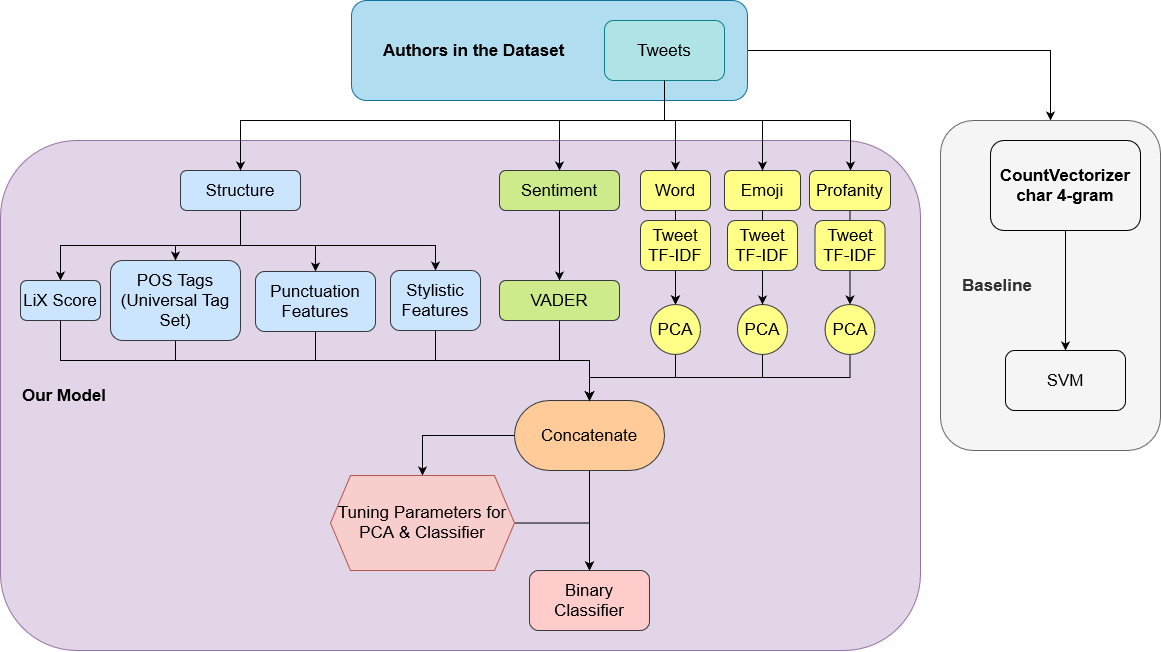
\includegraphics[width = \textwidth]{images/lang_proc.png}
        \caption{Final Model Used and Baseline Model representation}
        \label{fig:model_representation}
    \end{figure*}      
     \subsubsection{Misspelling}
    
    We thought that misspelling might be a good indicator of irony. By using PySpellchecker \footnote{\href{https://pyspellchecker.readthedocs.io/en/latest/}{PySpellchecker}} we found the misspelled words and set them in relation to the total number of words. However, it seems that the results greatly overlap for both classes and it is not a very practical feature for the classification. Because the misspellings did not add significant information, we did not use this feature out for our model training. We suspect that misspellings are in general very common on social media.
    % Use cross validation with the permutation_importance to average out the importance of different features
    % This is because different splits cause different features to be less or more important. 
    
    
    \subsubsection{Syntactic Complexity}
    
    Another type of feature we considered was syntactic complexity, which we hypothesized could be higher for non-ironic users.
    
    Syntactic complexity can be estimated in a number of ways including NP density, tree height and the number of high-level constituents per sentence \cite{barnwal2017using}. All of these approaches require parsing, which we did with \verb'spacy''s Dependency Parser\footnote{\url{https://spacy.io/usage/linguistic-features#dependency-parse}}. We tried implementing tree height, but the process proved very slow and expensive, and we dropped the feature so we could keep our model lightweight. We incorporate some syntactic information with POS counts, so it is not totally absent from our model.
